\chapter{\preliminary{Co-operative Memory Cache}}\index{memory cache}
\label{sct:crowd}
In order to replace the manually installed intermediate proxy servers, \cvmfs\ instances in the same subnet may co-operate in order to form a memory cache.
We propose a distributed algorithm to be implemented as {\scshape memcachd}~\cite{memcached04} client library to retrieve cached data from the memory of participating peers (cf.~Fig.~\ref{fig:memcached}).
\cvmfs\ instances running in a cluster shall thereby experience a greatly reduced access latency.
This system forms a cache layer on top.
It is fully decentralized and resilient to node churn.
It gathers and shares information about file presence in the local network.
Each peer can independently decide how much load it is willing to take.

\begin{figure}
	\begin{center}
		\begin{tikzpicture}
				\tikzset{
		thick,
		network/.style={draw,gray,thin}, 
		key/.style={anchor=west},
		action/.style={draw,red!60,very thick,->},
		background/.style={
			rectangle,
			fill=gray!10,
			inner sep=0.2cm,
			rounded corners=5mm}
	}
	  
	\node (switch) at (0,0) {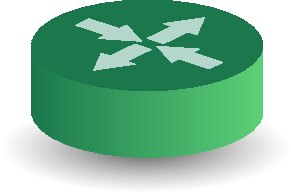
\includegraphics[width=2cm]{switch}};  
	\node (vm1) at (180:4cm) {
\includegraphics[width=2cm]{cvmfs-wo-memcached}};
	\node (vm2) at (225:4cm) {
\includegraphics[width=2cm]{cvmfs-wo-memcached}};
	\node (vm3) at (270:4cm) {
\includegraphics[width=2cm]{cvmfs-wo-memcached}};
	
	\node at (300:4.2cm) {$\bullet$};
	\node at (305:4.2cm) {$\bullet$};
	\node at (310:4.2cm) {$\bullet$};
	
	\begin{pgfonlayer}{background}
		\draw[network] (0,0) -- (node cs:name=vm1,angle=0);
		\draw[network] (0,0) -- (node cs:name=vm2,angle=90);
		\draw[network] (0,0) -- (node cs:name=vm3,angle=110);
	\end{pgfonlayer}

	\path (3.2cm,-0.2cm) node[anchor=east] (keytl) {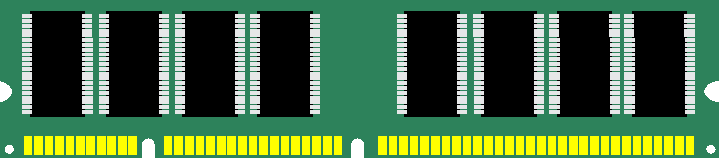
\includegraphics[height=0.3cm]{mem}} -- (3.45cm,-0.2cm) node[key]{memcached};
	\path (3.2cm,-1.1cm) node[anchor=east] (keybl) {
\includegraphics[height=0.9cm]{cvmfs}} -- (3.45cm,-1.1cm) node[key] (keybr) {CernVM-FS};
	\begin{pgfonlayer}{background}
        		\node[background, fit=(keytl) (keybl) (keybr)] {};
	\end{pgfonlayer}
			
	\node at (vm1) {
\includegraphics[width=2cm]{cvmfs-wi-memcached}};
	\node at (vm2) {
\includegraphics[width=2cm]{cvmfs-wi-memcached}};
	\node at (vm3) {
\includegraphics[width=2cm]{cvmfs-wi-memcached}};

			
	\node (vm1 cvmfs) at (node cs:name=vm1,angle=-15) {};
	\node (vm2 memcached) at ($(node cs:name=vm2,angle=60) - (0,0.2cm)$) {};
	\node (vm3 memcached) at ($(node cs:name=vm3,angle=60) - (0,0.2cm)$) {};
	\node (vm2 cvmfs) at (node cs:name=vm2,angle=-15) {};
	\draw[action,curve to,out=0,in=90] (vm1 cvmfs) to node[fill=white,near end] {store} (vm2 memcached);
	\draw[action,<-,curve to,out=90,in=0] (vm3 memcached) to node[fill=white,very near end] {retrieve} ($(vm3 memcached) + (-1cm,1cm)$) 
		to[out=180,in=0] (vm2 cvmfs);

		\end{tikzpicture}
	\end{center}
	\caption{Co-operative memory cache: Each node is extended by a {\scshape memcached} instance, steered by \cvmfs\ instances of neighbor nodes.}
	\label{fig:memcached}
\end{figure}

\section{The Algorithm}
We are seeking for a system where a client chooses its key space responsibility itself, according to how much load it is able to stand.
Instead of solving the load-balancing problem centrally, we want the peers to organize themselves.
Furthermore, in cases where a big bunch of peers joins or leaves simultaneously, we want the responsibilities to be rather stable.

We assume a set of peers that require certain data chunks over time.
Data chunks are identified by a key.
The key of a data chunk is considered to be a secure hash of the data chunk.
In contrast to the usual key-value store interface, we have immutable data and thus just a \texttt{get()} function.
Since we assume an outside channel from which we are able to retrieve chunks, new chunks are stored in the cache layer as a side effect of a cache miss.
In order to exchange requests and data, the peers send messages to each other.
The \texttt{request} message requests a certain chunk from another peer; it is answered by a \texttt{deliver} message that has the chunk as payload.
Figure~\ref{lst:impl} shows the implementation of the \texttt{get()} function and the \texttt{request} message handling.
Note that in case of a cache miss, the asked peer is responsible for retrieving the chunk via the outside channel.

Each peer maintains its own memory cache for data chunks, using a least recently used replacement strategy.
The peers may choose the size of their caches independently of each other.
Furthermore, each peer maintains $k$ \emph{slots}, for instance $k=16$.
A slot declares an area of responsibility within the key space.
This is done by a prefix of arbitrary length, \eg a slot $r$ with prefix 0x123 is responsible for chunks with keys starting with 0x123.
Other peers will ask the peer of slot $r$ for data chunks with keys starting with 0x123 except there is a slot having a longer matching prefix for a certain chunk.
If there are multiple such peers, they may ask any.

A slot can also be interpreted as node in the complete key space tree~(see Figure~\ref{fig:keyspace}).
In this representation, a slot is responsible for data chunks with keys in the subtree that is rooted at the slot's node.
In addition to its own slots, each peer keeps the information about the other peer's current slots.

\begin{figure}
	\begin{center}
		\resizebox{0.75\textwidth}{!}{%\documentclass[a4paper, 11pt]{article}\usepackage{tikz,ifthen}\usetikzlibrary{arrows,positioning,shapes,topaths,calc,fit,backgrounds,matrix,shadows,automata,patterns}\begin{document}

		\begin{tikzpicture}[shorten >=1pt,node distance=2cm,on grid,auto,
			edge/.style={->,color=gray},
			peer1/.style={color=blue!60,fill=blue!30,font=\large},
			peer2/.style={color=red!60,fill=red!30,font=\large},
			nopeer/.style={font=\large},
			key/.style={minimum size=5pt,node distance=0.75cm and 1.5cm}]
			
			\node[state, peer2] (p000) {000};
			\node[state, peer1] (p001) [right=of p000]{001};
			\node[state, nopeer] (p010) [right=of p001]{010};
			\node[state, nopeer] (p011) [right=of p010]{011};
			\node[state, nopeer] (p100) [right=of p011]{100};
			\node[state, nopeer] (p101) [right=of p100]{101};
			\node[state, peer2] (p110) [right=of p101]{110};
			\node[state, nopeer] (p111) [right=of p110]{111};
			
			\node[state, nopeer] (p00) at ($(p000) + (1,2)$) {00};
			\node[state, nopeer] (p01) at ($(p010) + (1,2)$) {01};
			\node[state, peer1] (p10) at ($(p100) + (1,2)$) {10};
			\node[state, peer1] (p11) at ($(p110) + (1,2)$) {11};
			
			\node[state, peer2] (p0) at ($(p001) + (1,4)$) {0};
			\node[state, nopeer] (p1) at ($(p101) + (1,4)$) {1};
			
			\coordinate (root) at ($(p011) + (1,6)$);
			\fill (root) circle (2pt);
			
			% Tree Edges
			\draw[edge] (root) --  (p0);
			\draw[edge] (root) --  (p1);
			\draw[edge] (p0) --  (p00);
			\draw[edge] (p0) --  (p01);
			\draw[edge] (p1) --  (p10);
			\draw[edge] (p1) --  (p11);
			\draw[edge] (p00) --  (p000);
			\draw[edge] (p00) --  (p001);
			\draw[edge] (p01) --  (p010);
			\draw[edge] (p01) --  (p011);
			\draw[edge] (p10) --  (p100);
			\draw[edge] (p10) --  (p101);
			\draw[edge] (p11) --  (p110);
			\draw[edge] (p11) --  (p111);
			
			\draw[->,very thick,curve to,out=0,in=100,color=red!60] (p0) to node {\large split} (p01) {};
			\draw[->,very thick,curve to,out=0,in=260,color=blue!60] (p10) to (p1) {};
			\draw[->,very thick,curve to,out=170,in=280,color=blue!60] (p11) to (p1) {};
			\node[color=blue!60] at ($(p1)-(0,2)$) {\large merge};
			
			% Key
			\node[state,key,peer1] (key peer1) at ($(p000) + (0,6)$) {};
			\node[key,anchor=west] at ($(key peer1) + (0.4,0)$) {\large Slots of peer A};
			\node[state,key,peer2,below=of key peer1] (key peer2) {};
			\node[key,anchor=west] at ($(key peer2) + (0.4,0)$) {\large Slots of peer B};
		\end{tikzpicture}
		
%\end{document}		
		}	
	\end{center}
	\caption{Example of a slot distribution over the key space $2^3$. There are 2 peers---peer A and peer B---having 3 slots each.}
	\label{fig:keyspace}
\end{figure}

In an ideal configuration with $n$ uniform peers, the sum of request for each peer's slots is the total amount of request divided by $n$.
The system seeks to come close to an ideal configuration.
To do so, each peer may perform two basic operations on its slots:
\begin{itemize}
	\item Merge --
		Two slots are merged in order to create a free slot.
		A peer always merges those two slots that have the smallest key space distance.
		The prefix of the resulting slot is decreased to the common prefix of the origin slots.
	\item Split --
		The slot's prefix length is increased by one bit, \ie the peer drops the right or the left subtree of the slot's key space.
		A peer decides which subtree to drop according to the resulting coverage of the key space tree.
		It looks for the largest subtree that is covered by another slot and drops that one.
\end{itemize}

New data chunks having a key that matches none of the slot prefixes occupy a new slot with the chunk's key as prefix.
A peer merges two slots when all its slots are already occupied.

Even though the slots with the smallest key distance are merged, a merge might produce rather big areas of responsibility.
Consider, e.\,g., the first merge of a peer with $k$ slots: two slots having complete keys as prefixes are merged.
If the keys are equally distributed, the resulting slot moves up from a leaf in the hash tree to a node at height $\log_2(k)$.

In order to restore the balance of the system, a peer seeks to split such an oversized slot.
We use the number of cache misses as an indicator for an oversized slot.
From our simulation experiments we know that a small constant parameter turns out to give good results; 
we currently choose to split after 3 cache misses.

Even without cache misses, a slot might turn out to be \emph{overloaded} in the sense that it has to serve more request than other slots.
This happens, for instance, for all the available slots at the moment when new peers join.
Let $r(s)$ be the number of requests for slot $s$.
Since a split drops half of the key space in responsibility, we split $s$ when $$r(s) > 2\frac{\sum_{\text{all slots $i$}} r(s_i)}{nk}$$

Conversely, a similar approach could avoid \emph{underloaded} slots by decreasing their prefixes.
But according to our simulation, such an approach decreases the quality of the algorithm.
It produces a lot more churn in the slot responsibilities, without changing the peers' hit rate significantly.

\begin{figure}[htbp]
	\centering
	\begin{algorithm2e}[H]
				\KwIn{Key $k$}
				\KwOut{Data chunk}
				\If{there is a matching slot}{
					$s$ $\leftarrow$ slot with a longest common prefix with $k$\;
					$p$ $\leftarrow$ peer of slot $s$\;
					\KwRet{$p$.request($k$, $s$)}\;
				}\Else{
					$c$ $\leftarrow$ retrieve chunk from outside channel\;
					Store $c$ in peer's cache\;
					\If{peer has a free slot}{
						$s$ $\leftarrow$ free slot\;
					}\Else{
						merge two of peer's slots\;
						$s$ $\leftarrow$ resulting free slot\;
					}
					prefix($s$) $\leftarrow$ $k$\;
					\KwRet{$c$}\;
				}
				\caption{get()}
				\label{alg:get}
			\end{algorithm2e}
	
	\begin{algorithm2e}[H]
				\KwIn{Key $k$, slot $s$}
				\KwOut{Data chunk}
				\If{peer has $k$ in its cache}{
					$c$ $\leftarrow$ corresponding data chunk
				} \Else{
					$c$ $\leftarrow$ retrieve chunk from outside channel\;	
					Store $c$ in peer's cache\;
					\If{number of cache misses > 3}{
						split($s$)\;	
					}
				}
				\If{number of requests for $s$ > 2 times slot request average}{
					split($s$)\;
				}
				sender.deliver($c$)
				\caption{request}
				\label{alg:request}
			\end{algorithm2e}
	\caption{Implementation of \texttt{get()} and \texttt{request}}
	\label{lst:impl}
\end{figure}	

\bigskip

In order to make accurate decisions, a peer needs some basic information about the system:
\begin{itemize}
	\item Which peers participate in the cache layer?
	\item What are the slot prefixes of the participating peers?
	\item What is the number of requests for the participating peers?
\end{itemize}

Overall, each peer has to maintain a couple of hundred bytes state per participating peer.
In our simulation, we just assume that this part of the global knowledge is available and up-to-date.
In a real system, this knowledge has to be exchanged among peers, which will introduce a certain delay.
We currently explore an approach that tackles this by a combination of multicast and gossip protocols.

\subsection{Load Balancing}
There is no particular load balancing mechanism included in our algorithm.
Instead, load balancing is a side effect of the algorithm and the nature of the CernVM-FS repositories.
Since almost all the files are relatively small and equal in size, 
we can reduce the general load balancing problem to an adequate distribution of the keys.
Each peer can then control its load by choosing the size of its memory cache freely and independently from all other peers.
Splitting and merging keeps the requests per slot equally distributed. 
Adjusting the slot size according to the number of cache misses controls the peer's load.

\section{Experimental Analysis}
\label{sec:simulation}
To judge our algorithm, we simulated our algorithm with a hand-written discrete event simulator based on both, application benchmark traces and synthetically generated traces.
The simulations are not supposed to provide an in-depth understanding of the algorithm.
Rather they are supposed to build a level of confidence in the algorithm's effectiveness to continue the analysis with an implemented prototype in real-world scenarios.
Our simulation does not take into account the latency amongst the peers nor the computation overhead.
This is negligible because the computation is marginal and we assume high-throughput low-latency communication between peers.
However, we do take into account the communication via the outside channel on a cache miss by a latency of 10\,ms.
We simulate up to 256 peers as a reasonable number for a single local subnet.

As stress test for the CernVM-FS we use software compilation, 
because several computing centers reported this as typical scenario.
Moreover, they observed that when multiple nodes in a cluster start to compile software, they easily turn down a standard NFS installation.

Thus, as a typical use case for the CernVM file system, we inspected the traces of compiling the example collection of the ATLAS experiment software~\cite{atlas05}.
The traces reflect 110\,000 requests of 1100 distinct files, \ie on average each file is opened 100 times.
The requests are not equally distributed but there are certain hot spots in time having the majority of requests.
Depending on the peer, the traces reflect a typical running time of a couple of hours.

We compare to two theoretical models, a large common LRU cache for all participating peers (\emph{idealistic case}) and small independent LRU caches for every peer (\emph{naive case}).
The combined cache size of all cache models is the same.
The efficiency gap of our algorithm compared to the idealistic is below 10\% for the ATLAS traces.
For synthetic traces, the efficiency of our algorithm tends to the idealistic case with increasing number of slots.
Naturally, with constant combined cache size and increasing number of peers the efficiency of the naive case drops.

\subsection{Load balancing}
For the ATLAS traces, half of the peers show a deviation of around 10\% from the mean in most cases, with the minimum and maximum being as far as 40\% from the mean.
Note that peers still have the option to decrease their load by decreasing the number of slots. 
We see furthermore that a peer is able to reduce its load by decreasing its cache size and/or number of slots.
The efficiency of the cache was not significantly reduced by high peer churn.
We observe, however, that loosing peers is more painful for the efficiency than the sudden arrival of new peers.
